
\documentclass[oneside]{normas-utf-tex} %oneside = para dissertacoes com numero de paginas menor que 100 (apenas frente da folha) 

% force A4 paper format
%\special{papersize=210mm,297mm}

\usepackage[brazil]{babel} % pacote portugues brasileiro
\usepackage[utf8]{inputenc} % pacote para acentuacao direta
\usepackage{amsmath,amsfonts,amssymb} % pacote matematico
\usepackage{graphicx} % pacote grafico
%\usepackage{times} % fonte times
\usepackage[final]{pdfpages} % adicao da ata
\usepackage{hyperref} % gera hiperlinks para o sumario, links, referencias -- deve vir antes do 'abntcite' 
\usepackage{tabularx}
\usepackage{pgfgantt}
\usepackage{rotating}
\usepackage[alf,abnt-emphasize=bf,bibjustif,recuo=0cm, abnt-etal-cite=2, abnt-etal-list=99]{abntcite} %configuracao correta das referencias bibliograficas.
\usepackage{subfigure}
\usepackage{xtab}
\usepackage{nomencl}
%\usepackage[portuguese,algoruled,longend,linesnumbered]{algorithm2e} %Para linhas numeradas e réguas de identação
\usepackage{algorithm2e}
\usepackage{listings}
% Definindo novas cores
\definecolor{verde}{rgb}{0.25,0.5,0.35}
\definecolor{jpurple}{rgb}{0.5,0,0.35}
% Configurando layout para mostrar codigos Java
\lstset{
  language=Java,
  basicstyle=\ttfamily\small,
  keywordstyle=\color{jpurple}\bfseries,
  stringstyle=\color{red},
  commentstyle=\color{verde},
  morecomment=[s][\color{blue}]{/**}{*/},
  extendedchars=true,
  showspaces=false,
  showstringspaces=false,
  numbers=left,
  numberstyle=\tiny,
  breaklines=true,
  backgroundcolor=\color{cyan!10},
  breakautoindent=true,
  captionpos=b,
  xleftmargin=0pt,
  tabsize=4
}
\renewcommand{\lstlistingname}{Código}
\renewcommand\lstlistlistingname{Lista de Códigos}
\newcommand*{\noaddvspace}{\renewcommand*{\addvspace}[1]{}}


% ---------- Preambulo ----------
\instituicao{Universidade Tecnol\'ogica Federal do Paran\'a} % nome da instituicao
\departamento{Departamento Acad\^{e}mico de Computa\c{c}\~ao} % nome do programa
\programa{Curso de Ci\^{e}ncia da Computa\c{c}\~ao} % área ou curso

\documento{Trabalho de Conclusão de Curso}
\nivel{Graduação}
\titulacao{Bacharel} 

\titulo{{Proposta de arquitetura de um sistema com base em OCR neuronal para resgate de caracteres em caixa de medicamento}} % titulo do trabalho em portugues
\title{\MakeUppercase{Character recognition of Mercosul Brazilian vehicle signs}} % titulo do trabalho em ingles

\autor{Fabiano Michel Gadenz} % autor do trabalho
\cita{GADENZ, Fabiano Michel} % sobrenome (maiusculas), nome do autor do trabalho

\palavraschave{reconhecimento, Mercosul, caracteres} % palavras-chave do trabalho
\keywords{recognize, Mercosul, Caracter} % palavras-chave do trabalho em ingles

\comentario{\UTFPRdocumentodata\ apresentado ao \UTFPRdepartamentodata\ da \ABNTinstituicaodata\ como requisito parcial para obten\c{c}\~ao do título de ``\UTFPRtitulacaodata\ em Computação''.}

\orientador{Prof. Dr. Everton Araújo de Coimbra} % nome do orientador do trabalho

\primeiroassina{Prof. Fulano\\ UTFPR - Câmpus Medianeira}
\segundoassina{Prof. Fulano\\ UTFPR - Câmpus Medianeira}
\terceiroassina{Prof. Fulano\\ UTFPR - Câmpus Medianeira}
\quartoassina{Prof. Fulano\\ UTFPR - Câmpus Medianeira}
\textoaprovacao{Este \UTFPRdocumentodata\ foi apresentado \`{a}s xx:xxh do dia X de mês de 20XX como requisito parcial para a obtenção do título de \UTFPRtitulacaodata~no \UTFPRprogramadata, da \ABNTinstituicaodata, Câmpus Medianeira. O candidato foi arguido pela Banca Examinadora composta pelos professores abaixo assinados. Após deliberação, a Banca Examinadora considerou o trabalho aprovado.}

\local{Medianeira} % cidade
\data{\the\year} % ano automatico

% desativa hifenizacao mantendo o texto justificado.
% thanks to Emilio C. G. Wille
\tolerance=1
\emergencystretch=\maxdimen
\hyphenpenalty=10000
\hbadness=10000
\sloppy

\definecolor{laranjautfpr}{cmyk}{0.0, 0.2, 1.0, 0.0}
\usepackage{enumitem}
\setlist{leftmargin=2cm}
\setlist{nosep}


%---------- Inicio do Documento ----------
\begin{document}


\capa % geracao automatica da capa
\folhaderosto % geracao automatica da folha de rosto

\termodeaprovacao

%resumo
\begin{resumo}
Incluir o resumo aqui para testes de bla bla bla bla Incluir o resumo aqui para testes de bla bla bla bla Incluir o resumo aqui para testes de bla bla bla bla Incluir o resumo aqui para testes de bla bla bla bla Incluir o resumo aqui para testes de bla bla bla bla
\end{resumo}

%abstract
\begin{abstract}
Include the abstract here Include the abstract here Include the abstract here Include the abstract here Include the abstract here Include the abstract here Include the abstract here Include the abstract here Include the abstract here Include the abstract here.
\end{abstract}

%------------------------DEDICATÓRIA------------------------------

\begin{dedicatoria}
Dedicatória do trabalho (opcional). 
\end{dedicatoria}

%-----------------------AGRADECIMENTOS----------------------------
\begin{agradecimentos}
Agradecimentos do trabalho (opcional). 
\end{agradecimentos}
%-----------------------EPÍGRAFE-----------------------------------
\begin{epigrafe}
Epígrafe do trabalho (opcional). 
\end{epigrafe}

\input{confListas}
\IfFileExists{/etc/resolv.conf}{}{\listadefiguras} %Geração de lista de figuras e automáticas
\IfFileExists{/etc/resolv.conf}{}{\listadetabelas} %Geração de lista de tabelas automáticas
% listas (opcionais, mas recomenda-se a partir de 5 elementos)
%\listadequadros % geração automatica da lista de quadros
\listadesiglas % geracao automatica da lista de siglas
%\listadesimbolos % geracao automatica da lista de simbolos

% sumario
\sumario % geracao automatica do sumario


%---------- Inicio do Texto ----------
% recomenda-se a escrita de cada capitulo em um arquivo texto separado (exemplo: intro.tex, fund.tex, exper.tex, concl.tex, etc.) e a posterior inclusao dos mesmos no mestre do documento utilizando o comando \input{}, da seguinte forma:

%\setcounter{page}{48}

\setlength{\parskip}{0.0cm}
\chapter{Introdução}\label{ch:intro}

As instruções fazem parte do nosso aprendizado e nos levam a efetuarmos atitude corretas. Para evitar sérias consequuencias ao usuário, a correta realizacão de uma tarefa depende da legibilidade das informações fornecidas e da qualidade da representação gráfica das mesmas \cite{FUJITA2007}.


No caso dos medicamentos, as informações descritas na bula são imprescindíveis para o ser humano, pois desempenham um papel fundamental durante o processo de tratamento do mesmo. Segundo Fujita & Spinillo \cite{FUJITA2006}, a apresentação gráfica do conteúdo informal nas bulas de remédios influencia sua leitura e compreensão. Deficiências tanto ao nível de conteúdo com uma linguagem muito formal, quanto na apresentação gráfica das informações em bulas como por exemplo a pequena fonte encontrada, pode ser levado ao mau uso de medicamentos, comprometendo a saúde e até acarretando sérias consequencias na saúde do indivíduo, principalmente para os idosos, muitas vezes com limitações motoras ou limitados de informação, devido a idade. 



Considerando a importância da leitura das bulas e da difícil compreensão de seu conteúdo para o uso correto e seguro de medicamentos, o presente trabalho visa identificar padrões de imagens com técnicas de processamento de imagem (\sigla{PDI}{Processamento de Imagem})  e um estudo entre métodos de reconhecimento ótico de caracteres (\sigla{OCR}{Reconhecimento Ótico de Caracteres}) embarcados no celular, com intenção de melhorar o poder acertivo de métodos de OCR com técnicas de PDI para corrigir a perspectiva da imagem, com a finalidade de identificar o medicamento através de uma foto capturada por meio de um telefone celular da embalagem do medicamento.




\section{Objetivo Geral e específico}
Voltado ao problema da difícil leitura de bula  de medicamento da população brasileira, o objetivo deste trabalho é a apresentação de uma proposta de arquitetura baseada em métodos de processamento de imagem, que possa contribuir para a leitura de métodos OCR processados diretamente pelo aparelho celular.
Este trabalho apresenta um aplicativo \textit{mobile} envolvendo as tecnologias de PDI, OCR com processamento inteiramente no dispositivo móvel. Entre essa proposta apresentada, é preciso desenvolver tais técnicas:

\begin{itemize}
  \item Criar uma base de imagens de bulas e caixas de medicamentos.
  \item Métodos de pré processamentos, como por exemplo, técnicas de iluminação, redução de ruídos e perspectiva da imagem capturada.
  \item Comparar o OCR da Google com e sem as técnicas de processamento de imagem.
  \item Apresentar informações detalhadas do medicamento inspecionado na foto para fácil entendimento de um usuário leigo e também para um agente da saúde.
\end{itemize}



\section{Justificativa}
O crescimento da população de idosos é um fenômeno mundial e está ocorrendo a um nível sem precedentes. Segundo dados do Instituto Brasileiro de Geografia e Estatística (\sigla{IBGE}{Instituto Brasileiro de Geografia e Estatística}), em 2012, o grupo das pessoas de 60 anos ou mais representava 12,8 porcento da população brasileira residente, porém, em 2017, esse percentual cresceu para 14,6 porcento \cite{jornaldocomercio1}.


Devido às dificuldades de leitura e entendimento das bulas de medicamentos relatadas por leitores e usuários, a Agência Nacional de Vigilância Sanitária (\sigla{ANVISA}{Agência Nacional de Vigilância Sanitária}), órgão brasileiro do Ministério da Saúde, implementou em 19 de janeiro de 2010 a Resolução RDC nº. 47/2009 que estabelece regras para elaboração, harmonização, atualização, publicação e disponibilização de bulas de medicamentos para pacientes e para profissionais da saúde \cite{PORTALANVISA2019}.










\chapter{FUNDAMENTAÇÃO TEÓRICA} \label{cap:funda}

Nessa seção é descrito o estado da arte do tema escolhido. Primeiramente é dado uma breve introdução sobre processamento de imagem, dando maior ênfase no processo de análise de imagem, seguindo teoria de \citeonline{GONZALEZ1992}. Este capítulo também será utilizado para descrever o funcionamento de um sistema OCR.

\section{Processamento Digital de Imagens}


Segundo \citeonline{Huang1996} visão computacional possui um propósito duplo. Partindo de um ponto de vista biológico, visão computacional é o estudo dos modelos computacionais do sistema visual humano. Já partindo de um ponto de vista de engenharia, visão computacional tem o objetivo de criar sistemas autônomos capazes de executar tarefas que o sistema visual humano executa, e em alguns casos até supera.


Para \citeonline{PEDRINI2008}, a visão computacional pode ser dividida em dois níveis de abstração: processamento de imagens (baixo nível) e análise de imagens (alto nível). O processamento digital de imagens pode ser determinado como um conjunto de técnicas para capturar, representar e transformar imagens utilizando um computador. A aplicação dessas técnicas permite extrair e identificar informações das imagens e melhorar a qualidade visual de aspectos estruturais, simplificando a percepção humana e a interpretação automática por meio de máquinas \cite{PEDRINI2008}. Essa abordagem, de baixo nível, utiliza técnicas como o aumento de contraste, a redução de ruído, a extração de bordas e a compressão de imagens.

De acordo com \citeonline{GONZALEZ2002}, a área de PDI vem evoluindo constantemente no decorrer dos anos, com uma ampliação significativa dos estudos envolvendo morfologia matemática, redes neurais, processamento de imagens coloridas, compressão de imagens, reconhecimento de imagens e sistemas de análise de imagens baseados em conhecimento.


O objeto de operação do Processamento Digital de Imagens são as imagens digitais. Uma imagem na forma digital é representada por meio de matrizes, as quais mapeiam as cores reais da imagem, do mundo físico para o digital \cite{Almeida2018}.





Os sistemas de PDI consistem em um conjunto de técnicas que possibilitam a captura de imagens por meio de equipamentos variados, como tomógrafos médicos, câmeras fotográficas, satélites e outros, tal como a representação e transformação destas imagens. O propósito é fazer a extração e identificação das informações que fazem parte das imagens, de forma automática por meio de máquinas \cite{PEDRINI2008}.

% EM TODAS AS SEÇÕES VOCÊ DEVERÁ TRAZER ARTIGOS QUE APLICARAM OS TEMAS DAS SEÇÕES E COMENTAR SOBRE O OBJETIVO E RESULTADO OBTIDOS NESTES TRABALHOS.
%fabiano: tentei encaixar autores relevantes em muitas afirmações. está faltando algum?

% EVERTON: Veja a seção 2.1. Você apenas referenciou o tema. É importante que você traga artigos onde o tema da seção foi utilizado e aplicado, trazendo a colaboração e resultado do artigo. Por exemplo> fulano de tal utilizou tal coisa e em seus estudos foi possível ..... É preciso ter referencial assim para todas as suas fundamentações.


\subsection{Representação de Imagens Digitais}
% EVERTON: Você fala sempre deste Gonçalves, não tem outras fontes? Para não ficar direcionado? Talvez buscar por quem tenha utilizado trabalho dele também. Quando se refere a elementos de uma função, coloque em itálico: m, n, M, N, f(x,y)....

Segundo \citeonline{Goncalves2016}, uma imagem pode ser representada no plano cartesiano por uma função f(x,y), onde x e y são coordenadas espaciais. A função f(x,y) possui, comumente, um valor em níveis de cinza, ou cor, em qualquer ponto da imagem. O ponto de origem representado pela coordenada (0,0) fica situado no canto superior esquerdo da imagem.




A Figura \ref{img1} ilustra como seria um imagem digital em forma de notação matricial. Os elementos dessa matriz são chamados de elementos pictóricos, elementos de imagens, pels e pixel. O \textit{Pixel} (contração de Picture element) é o termo mais utilizado \cite{GONZALEZ2006}. O índice m representa a linha na qual o pixel se encontra, enquanto que o índice n aponta a coluna na qual está localizado o pixel. Em uma imagem M linhas e N colunas, m terá seu valor variando de 0 até M-1 e n terá seu valor variando de 0 até N-1 \cite{Almeida2018}. 

 \begin{figure}[h!]
	\centering
	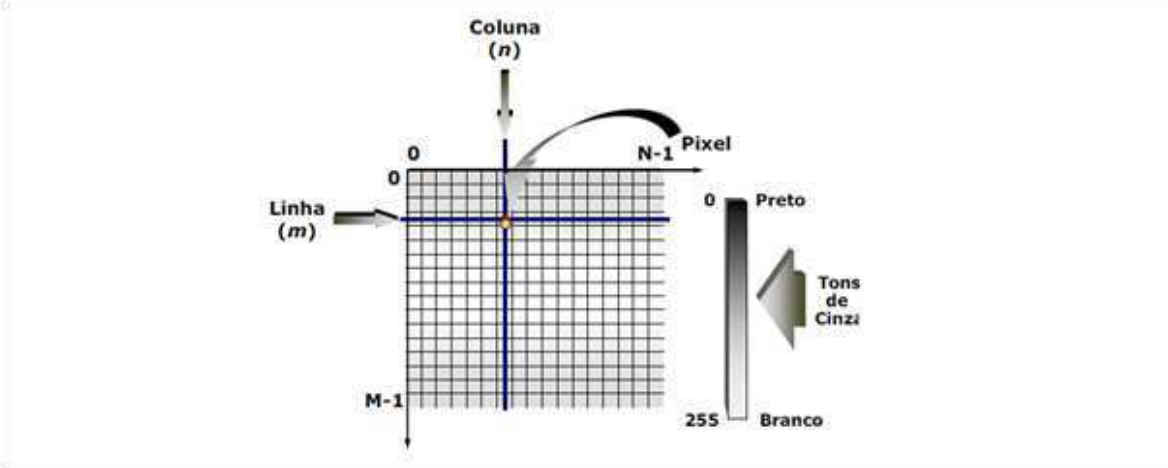
\includegraphics[width=0.85\textwidth]{Imagens/imagem1} 
	\caption[Representação da imagem em uma matriz bidimensional.]{Representação da imagem em uma matriz bidimensional.}
\fonte{\citeonline{Goncalves2016}}
	\label{img1}
\end{figure}

Segundo \citeonline{PEDRINI2008} uma imagem digital pode ser representada por meio de uma matriz bidimensional, na qual cada pixel da imagem corresponde a um elemento da matriz. Na Figura 2 é possível ver um exemplo de representação matricial de uma imagem, sendo que uma pequena região destacada é formada por números inteiros que representam o nível de cinza dos pixels da imagem. Existem várias vantagens ao utilizar matrizes para representação de imagens, pois são estruturas simples para armazenar, manipular e visualizar dados \cite{PEDRINI2008}. 

 \begin{figure}[h!]
	\centering
	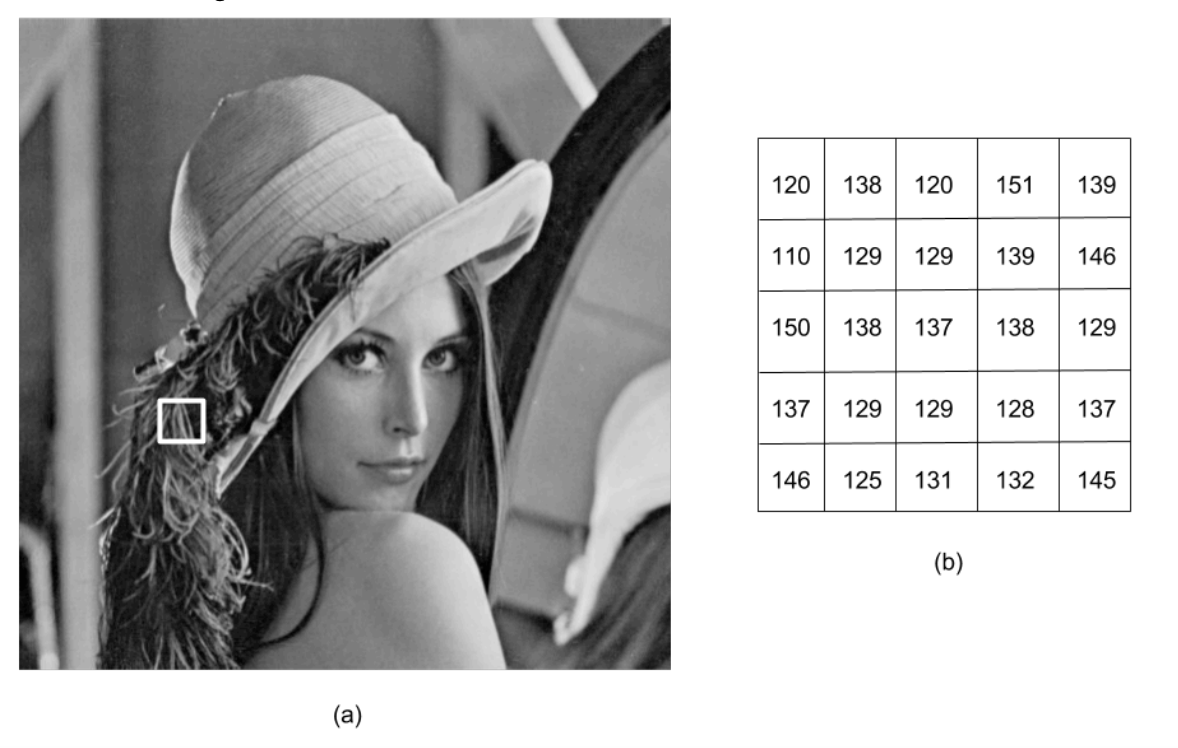
\includegraphics[width=0.7\textwidth]{Imagens/imagem6} 
	\caption[Representação matricial;]{Representação matricial; (a) imagem; (b) níveis de cinza correspondentes a região
destacada da imagem.}
\fonte{\citeonline{PEDRINI2008}}
	\label{fig:tux_laplace}
\end{figure}


Em uma imagem digital existem vários relacionamentos importantes entre os pixels. Conforme descrito em \citeonline{GONZALEZ2002}, 
um pixel p de coordenadas (x,y) possui uma vizinhança horizontal e vertical determinadas por (x-1, y), (x+1, y) e (x, y-1), (x, y+1) denominada vizinhança-4, e também uma vizinhança diagonal composta pelas coordenadas (x-1, y-1), (x-1, y+1), (x+1, y-1) e (x+1, y+1), convencionado com o nome de vizinhança-8 a união destas vizinhanças.

Quando o pixel p estiver localizado na borda da imagem, alguns dos pixels vizinhos não estarão presentes na imagem. Isto pode ser mais bem entendido analisando-se a Figura 3 que demonstra visualmente o conceito de vizinhança de um pixel.

 \begin{figure}[h]
	\centering
	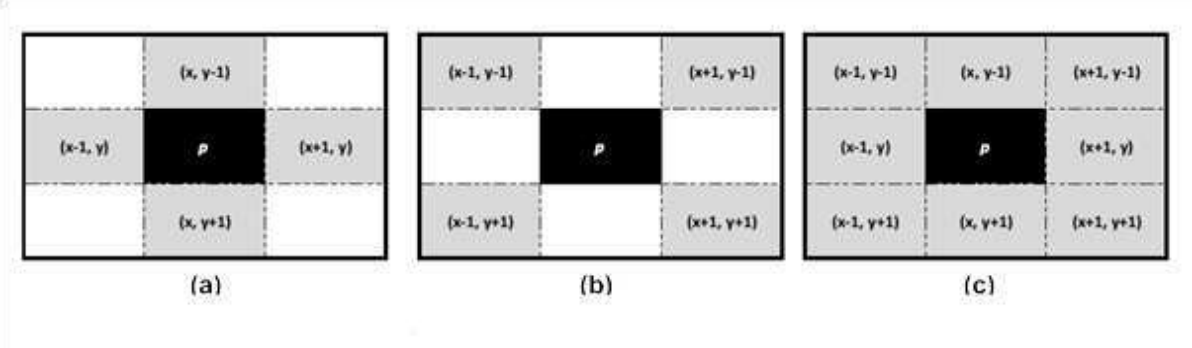
\includegraphics[width=1.0\textwidth]{Imagens/imagem3} % <- formatos PNG, JPG e PDF
	\caption[Texto que vai aparecer na lista de fig.]{Tipos de vizinhança. (a) Vizinhança-4; (b) Vizinhança diagonal; (c) Vizinhança-8.  (a) Imagem; (b) Histograma.}
\fonte{\citeonline{Goncalves2016}}%citaç\~ao do livro onde pegou a figura	
	\label{fig:tux_laplace}
\end{figure}

A conectividade entre pixels é um conceito importante no processamento de imagens, em especial para o reconhecimento de bordas de objetos presentes em uma imagem. Para identificar se dois pixels são conexos, é preciso averiguar se são vizinhos e se seus níveis de cinza são similares \citeonline{Goncalves2016}. É fundamental analisar a possibilidade de haver conexidade por meio da utilização da vizinhança-4 ou utilizando a vizinhança-8.




\section{Ciclo de Gonzalez}
%EVERTON: Veja a data da sua referência quando fala das últimas décadas. Tem um comentário do PEDRO no meio do texto
Os dispositivos desempenham um papel essencial em um sistema de processamento de imagem, podendo ser utilizados para aquisição, armazenamento, processamento, transmissão e exibição de imagens. Com o crescente avanço tecnológico e a demanda de certas áreas de aplicação, estes dispositivos têm evoluído de forma significativa nas últimas décadas \cite{PEDRINI2008}.
(PEDRO: atualizar imagem conforme livro de 2018)

Segundo \citeonline{GONZALEZ1992}, as técnicas em análise de imagem podem ser divididas em três áreas básicas: (1) aquisição e processamento de baixo nível, com funções que podem ser vistas como reações automáticas, ou seja, reações que não requerem comportamento inteligente; (2) processamento de nível intermediário, com processos de extração e caracterização de componentes em uma imagem; e (3) processamento de alto nível, que envolve os processos de reconhecimento e interpretação. A Figura 3 mostra os processos de cada uma dessas áreas.



 \begin{figure}[h]
	\centering
	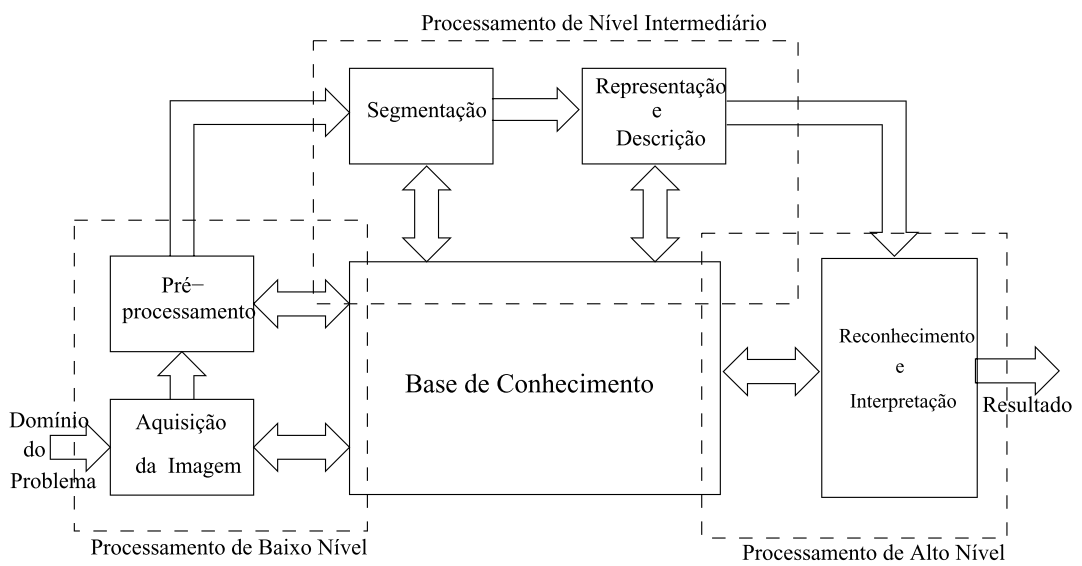
\includegraphics[width=1.0\textwidth]{Imagens/imagem5} % <- formatos PNG, JPG e PDF
	\caption[Elementos do processo de análise de imagem.]{Elementos do proceso de análise da imagem. }
\fonte{\citeonline{GONZALEZ1992}}%citaç\~ao do livro onde pegou a figura	
	\label{fig:tux_laplace}
\end{figure}



% EVERTON: cuidado que daqui pra frente está parecendo metodologia, como se faz. Aqui é referencial teórico
O primeiro passo do processo de reconhecimento é a aquisição da imagem. Segundo \citeonline{GONZALEZ1992}, o primeiro passo do processo requer apenas um sensor de imagens e a capacidade para digitalizar o sinal produzido pelo
sensor. O sensor converte a informação óptica em um sinal elétrico e o digitalizador transforma a imagem analógica em imagem digital. A imagem resultante pode apresentar diversas imperfeições, tais como: presença de pixels ruidosos, contraste e/ou brilho inadequado, etc (MARQUES;VIEIRA, 1999).

Após a aquisição e digitalização da imagem, o próximo passo é o pré-processamento. A função chave do pré-processamento é melhorar a imagem, com o objetivo de aumentar as chances de sucesso dos processos seguintes \cite{GONZALEZ1992}. Nesta etapa, são utilizadas técnicas para aumento de contraste, remoção de ruídos, realce e normalização, com o objetivo de converter os padrões para uma forma que possibilite uma simplificação do processo de reconhecimento \cite{Rodrigues2002}.

O próximo estágio é o processo chamado de segmentação. A segmentação de imagens, demonstrado na figura X consiste em dividir uma imagem em suas unidades significativas, para uma melhor caracterização das regiões de interesse (\sigla{ROI}{Região de Interesse}). As operações de segmentação procuram isolar regiões de pontos da imagem pertencentes a objetos, para posterior extração de atributos \cite{Lourdes2010}.
 \begin{figure}[h]
	\centering
	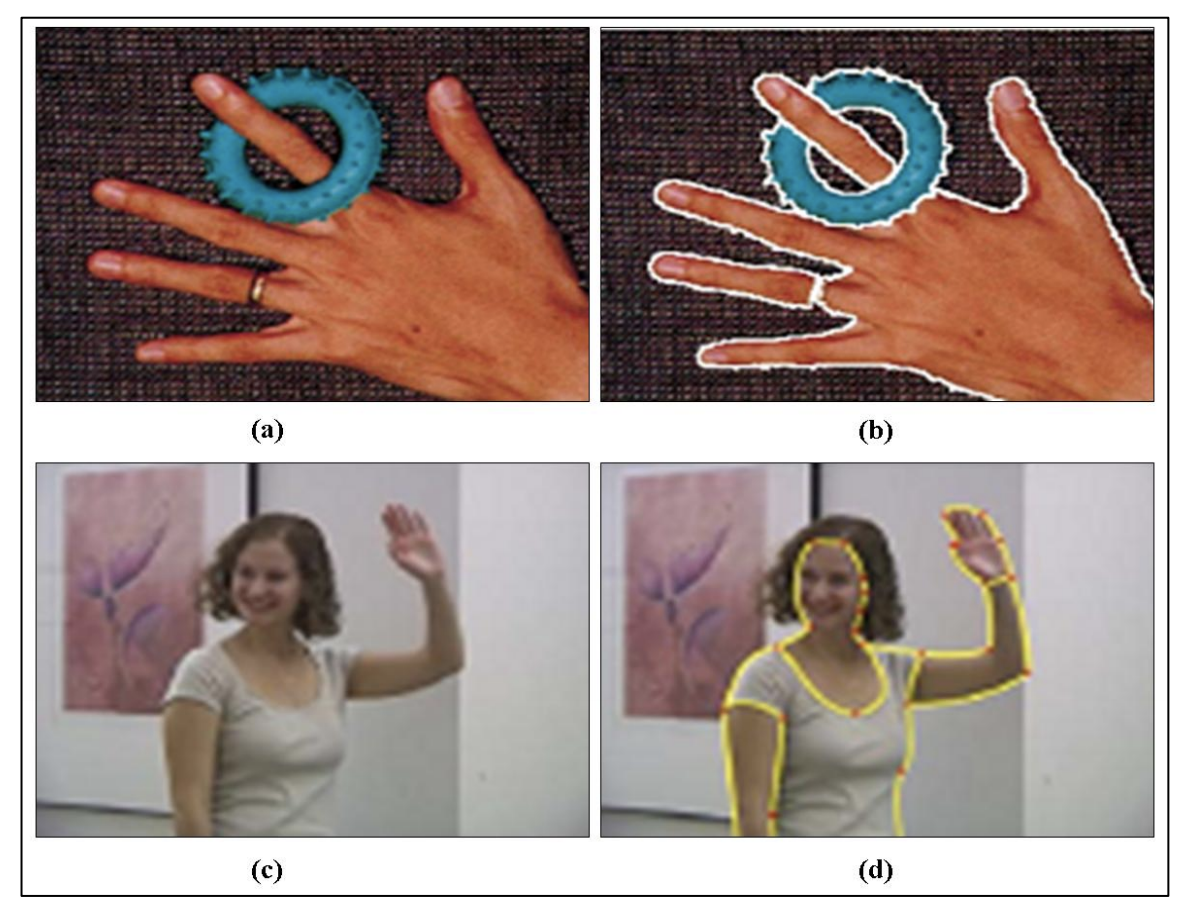
\includegraphics[width=1.0\textwidth]{Imagens/segmentacao} % <- formatos PNG, JPG e PDF
	\caption[Segmentação de Imagens: (a) imagem original, (b) imagem após segmentação; (c) imagem original; (d)imagem após segmentação.]{Segmentação de Imagens: (a) imagem original, (b) imagem após segmentação; (c) imagem original; (d)imagem após segmentação.}
\fonte{\citeonline{SZELISKU2010}}%citaç\~ao do livro onde pegou a figura	
	\label{fig:tux_laplace}
\end{figure}
De um modo geral, as técnicas de segmentação utilizam duas abordagens principais: a similaridade entre os pixels e a descontinuidade entre eles. A binarização de imagens, técnica baseada em similaridade, é a técnica mais utilizada, é uma  simples e eficiente técnica do ponto de vista computacional, sendo portanto comumente utilizada em sistemas de visão computacional \cite{ISRAEL2003}.

Na segmentação com descontinuidade entre os pixels, a segmentação é baseada nas técnicas de limiarização, crescimento por regiões, união e divisão de regiões \cite{Rodrigues2002}.  % VEJA QUE AQUI E EM OUTROS PONTOS VOCÊ TRAZ TERMOS ESPECÍFICOS, QUE PODERIAM SER EXPLICADOS EM SEU TEXTO.

A etapa de segmentação é seguida por ima etapa de representação e descrição, na qual, através de descitores, busca-se obter um conjunto de dados correspondentes àquela imagem.

Normalmente, após a segmentação, dados brutos de pixel são obtidos. Por consequência, pode ser fundamental o processo de converter os dados para uma forma apropriada, possibilitando o processamento digital. 

Dois tipos de representação podem ser utilizados: representação limite ou representação regional. Quando o foco está com características de localização nas extremidades, como por exemplo cantos e bordas da imagem, é apropriada a representação limite. Representação regional é apropriada quando o foco está localizado no centro da imagem e é possível encontrar uma vizinhança-8. Escolher a representação é apenas uma parcela da solução para a conversão de dados brutos em uma forma adequada para o processamento computacional. \cite{Rodrigues2002}
%EVERTON: Estou preocupado com a época das referências. São muito antigas. Nada mudou neste período?

O ultimo estágio no processo de análise da imagem envolve reconhecimento e interpretação. Reconhecimento é o processo que fixa um rótulo a um objeto baseado na informação extraída na etapa anterior. Interpretação envolve a fixação de significado a um grupo de objetos reconhecidos. Para resolver problemas de reconhecimento pode-se partir de três abordagens: estatística, estrutura e neural \cite{GONZALEZ1992}.

Todas as etapas descritas pressupõem a existência de um conhecimento sobre o problema a ser resolvido, armazenado em uma base de conhecimento, cujo tamanho e complexidade podem variar enormemente. Idealmente, esta base de conhecimento deveria não somente guiar o funcionamento de cada etapa, mas também permitir a realimentação entre elas, \cite{marques1999}.


\section{Detecção de Bordas}

Segundo \citeonline{Antonio}, uma borda é definida por uma mudança repentina do nível de cinza, ou seja ocorre uma descontinuidade no tom de cinza. Dessa forma, a descontinuidade pode ser percebida quando o gradiente da imagem tem uma brusca variação. Para \citeonline{PEDRINI2008}, a detecção de bordas é o limite entre duas regiões com propriedades razoavelmente distintas de nível de cinza. \citeonline{SZELISKU2010}, define que uma borda é uma fronteira entre regiões de diferentes cores, intensidades ou texturas. Já \citeonline{marques1999} definem borda como uma descontinuidade na luminosidade de uma imagem.

Para \citeonline{Silva2001}, é possível considerar o pixel como borda calculando o gradiente deste pixel e, caso o gradiente seja maior do que um valor de limiar pré-definido, o pixel é considerado como borda. 

Para \citeonline{GONZALEZ2002}, a idéia associada à maioria das técnicas para a detecção de bordas é o cálculo de um operador local diferencial que seja sensível a mudanças ou descontinuidade nos níveis de cinza. Um operador de derivada pode ser usado para executar essa função, visto que se poderia avaliar a taxa de mudança da função dos níveis de cinza. A taxa de mudança dos níveis de cinza em uma imagem tende a ser maior perto das bordas e menor em áreas constantes, caracterizando as bordas como os pontos máximos da derivada \cite{PEDRINI2008}.

Segundo \citeonline{Franco2013}, diversas abordagens foram propostas ao longo dos anos para a detecção de bordas em imagens digitais, como por exemplo, os operadores de Roberts, Hough, Sobel e Canny. A abordagem utilizada nesse trabalho é a transformada de Hough. Segundo \citeonline{PEDRINI2008}, o método de Hough é altamente eficiente na detecção de bordas em linhas retas.
%EVERTON: A abordagem utilizada nesse trabalho é a transformada de Hough isso deverá estar no MATERIAL E MÉTODOS se for sobre seu trabalho.

Na detecção de linhas retas, \citeonline{SZELISKU2010} diz que parte da complexidade inerente à detecção de linhas retas em imagens vem do fato de que, no mundo real, as linhas são normalmente compostas por componentes desconectados ou mesmo feitas de diversos segmentos colineares, sendo necessário agrupá-los para possibilitar a detecção. Em diversas áreas de PDI surge o problema da determinação da localização e orientação de linhas retas em imagens.
%EVERTON: O texto Em diversas áreas de PDI surge o problema da determinação da localização e orientação de linhas retas em imagens. parece largado. Sem ligação com o que vinha sendo dito.

\citeonline{PEDRINI2008} citam que o problema na detecão de linhas retas consiste essencialmente em achar subconjuntos de pontos que sejam colineares e que o método conhecido como Transformada de Hough é eficiente nesta tarefa. A transformada de Hough vem sendo usada para esta finalidade em imagens binárias, onde seu princípio básico é a conversão de coordenadas de um ponto no plano cartesiano em parâmetros em que descrevem este ponto em termos de inclinação e distância de um ponto de origem.


A transformada de Hough é capaz de detectar grupos de pixels que pertencem a uma linha reta (mesmo que esteja quebrada e/ou com ruídos). Uma linha reta é geralmente descrita como y = mx + b. As características desta reta são a inclinação m e a intersecção b. Assim, uma reta y = mx + b pode ser representada como um ponto (b, m) no espaço dos parâmetros \cite{HOUGHKIM}. 

Porém, ambos parâmetros são ilimitados, isto é, à medida em que a reta torna-se vertical, as magnitudes de b e m tendem ao infinito. Para um bom desempenho computacional, é melhor parametrizar as retas usando dois outros parâmetros, assim transformando a equação da reta na forma polar $(\theta, \rho)$, dada a Equação~\ref{eq:eqreta},

\begin{equation}
\rho = x*\cos{\theta} + y*\sin{\theta}
\label{eq:eqreta}
\end{equation}

$(\rho)$ é a distancia perpendicular da origem (0,0) à reta e $(\theta)$ é o angulo formado entre a reta perpendicular e o eixo x, o espaço $(\theta, \rho)$ deve ser discretizado de modo a permitir sua implementação conforme Figura 6. Como $(\theta)$ é medido em relação ao eixo x, os valores possíveis variam de 0$^{\circ}$ a 180$^{\circ}$ e uma discretização com incremento de 1$^{\circ}$ deixaria 181 angulos possíveis \cite{PEDRINI2008}.

De acordo com \citeonline{GONZALEZ2002}, as principais vantagens da transformada de Hough é que mesmo segmentos que apresentem regiões obstruídas por outros objetos podem ser detectados, e sua baixa sensibilidade à ruído, já que os pontos de uma imagem corrompidos por esse ruído dificilmente serão mapeados em uma mesma célula de acumulação.

 \begin{figure}[h]
	\centering
	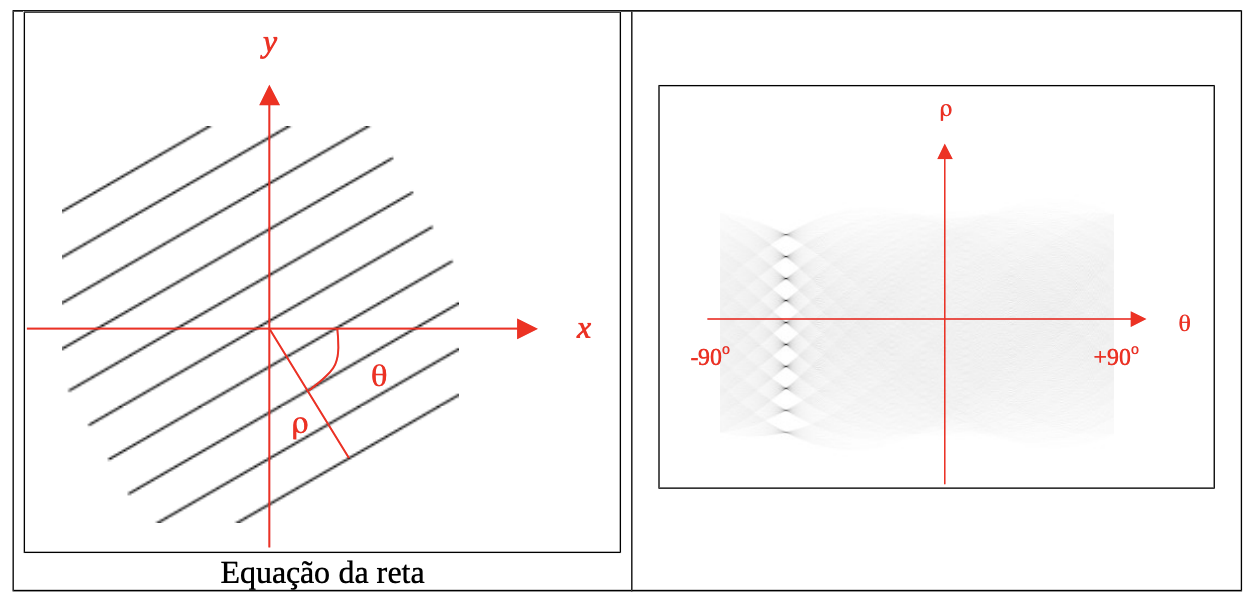
\includegraphics[width=1.0\textwidth]{Imagens/eqreta} 
	\caption[Representação de uma reta através de coordenadas polares.]{Representação de uma reta através de coordenadas polares.}
\fonte{\citeonline{HOUGHKIM}}	
	\label{fig:tux_laplace}
\end{figure}


\section{Correção de Perspectiva}

Segundo \citeonline{Silveira2006}, a distorção da imagem ocorre devido a diferentes aspectos durante sua captação. A distância entre o plano do objeto e o capturador de imagens promove um erro de perspectiva. Esse tipo de erro pode ser minimizado por meio do posicionamento do segmento de interesse próximo à tela. A correção de erros de perspectiva é desenvolvida por métodos geométricos de relativa simplicidade e vem sendo amplamente utilizada em imagens de raio x. Indo na direção de estruturas de menor escala, a correção de perspectiva é aplicada em processos de digitalização de documentos, onde a correção de distorções na imagem, acarreta em uma maior capacidade de reconhecimento de caracteres em um texto digitalizado \cite{Pereira}. 

A imagem 7 mostra dois exemplos de imagens distorcidas, capturadas por uma câmera digital de baixa resolução e suas respectivas correções. Há uma grande variedade de programas e aplicativos capazes de corrigir as distorções de perspectiva em imagens. Ainda que os programas consigam corrigir as distorções por perspectiva de maneira satisfatória, a correção não se dá em tempo real, além de requerer uma interface gráfica com o usuário para que a correção seja feita.
 \begin{figure}[!h]
	\centering
	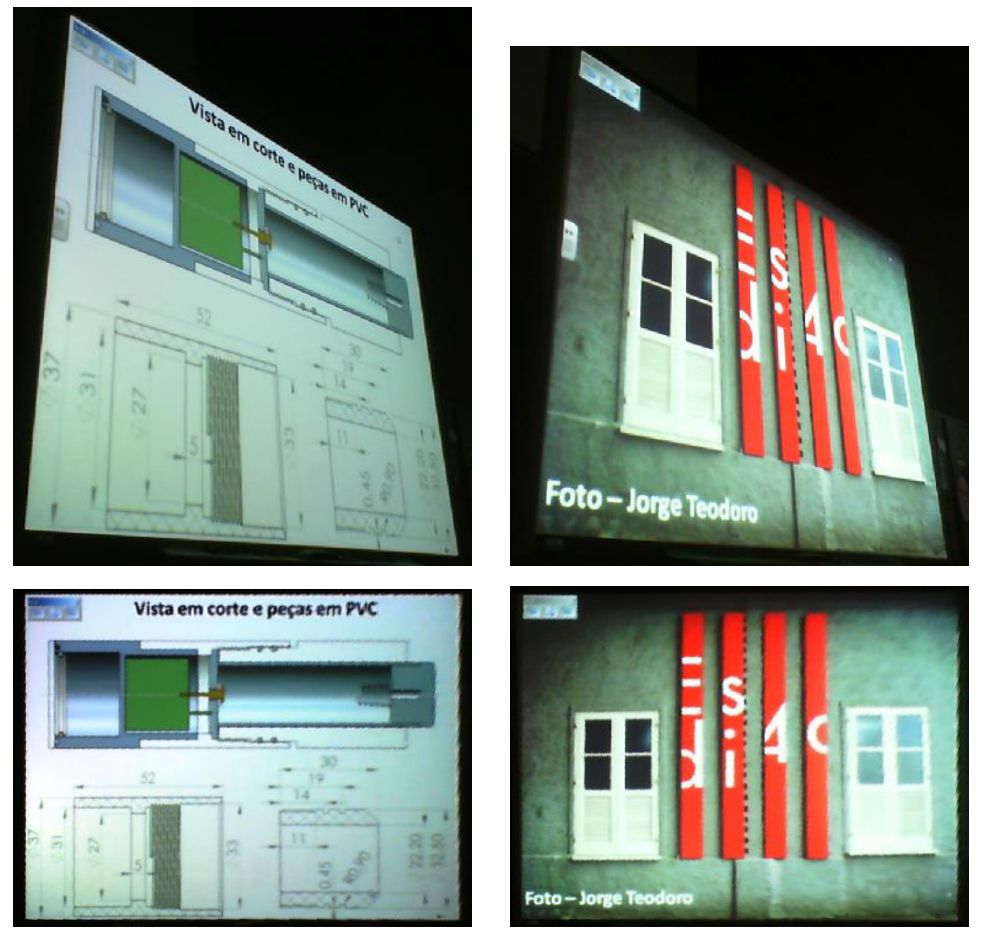
\includegraphics[width=1.0\textwidth]{Imagens/imagensdistorcidas} 
	\caption[Imagens distorcidas e corrigidas.]{Imagens distorcidas (acima) e corrigidas (abaixo).}
\fonte{\citeonline{Pereira}}	
	\label{fig:tux_laplace}
\end{figure}

\citeonline{ZHANG2007} Abordam uma proposta de automatização de correção de imagens fotográficas de quadros brancos.A detecção dos limites formados pelo quadrilátero de uma projeção ou de um quadro branco é o principal obstáculo para a realização de um sistema automatizado de correção de distorções de perspectiva. Os procedimentos descritos por \citeonline{ZHANG2007} são mostrados na Figura 8, onde a transformada de Hough é usada para a detecção dos limites do quadro ou projeção.

 \begin{figure}[h]
	\centering
	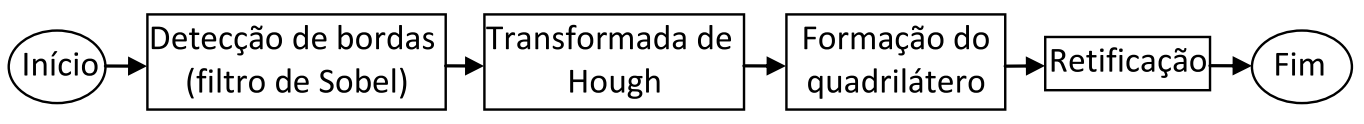
\includegraphics[width=1.0\textwidth]{Imagens/metodologiacorrecao} 
	\caption[Metodologia de detecção.]{Metodologia de detecção.}
\fonte{\citeonline{Pereira}}	
	\label{fig:tux_laplace}
\end{figure}

A detecção do contorno de uma imagem está sujeita às condições de luminosidade do ambiente que podem impor limites na detecção automática do contorno, um algoritmo de detecção de contorno deve apresentar boa imunidade a variações de iluminação do ambiente. \cite{Pereira}.

%//TODO estudos nao finalizados. tópico importante: four_point_transform

\section{RECONHECIMENTO ÓPTICO DE CARACTERES (OCR)}
Reconhecimento óptico de caracteres (OCR) é uma tecnologia que utiliza mecanismos de aquisição, tais como câmeras fotográficas, filmadoras e afins para capturar imagens e posteriormente realizar processamentos nestas para reconhecer caracteres alfanuméricos presentes. Essa tecnologia tenta se aproximar do sistema visual humano, porém ainda não é capaz de competir com a capacidade de leitura deste \cite{Mithe2013}.

 Existem diversas técnicas de identificação automática, na qual cada uma satisfaz às necessidades de sua área de aplicação. Reconhecimento de voz, tarja magnética, código de barra, impressão digital e OCR são exemplos de aplicações que utilizam tecnologias de identificação automática. Segundo \citeonline{Bhatia2014}, os sistemas de OCR são aqueles capazes de transformar uma grande quantidade de documentos, tanto impresso como manuscrito, em texto de máquina codificado. O reconhecimento de caracteres pode ser desempenhado off-line, onde ocorre após a escrita ou impressão do documento estiver finalizada, porém o reconhecimento também pode ser on-line onde o computador reconhece os caracteres na maneira que eles vão sendo desenhados \cite{Eikvil1993}. A Figura 9 mostra as possíveis etapas para o reconhecimento de caracteres.

%EVERTON: Troque no parágrafo anterior a palavra desempenhado. Seria realizado?
 \begin{figure}[h]
	\centering
	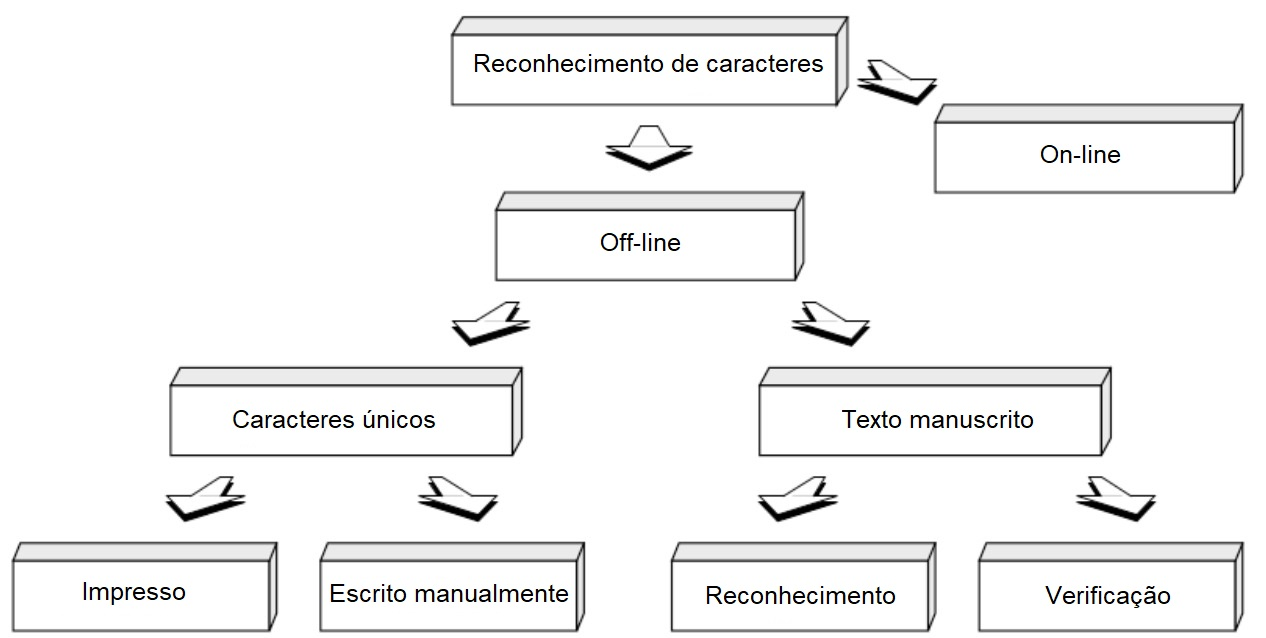
\includegraphics[width=1.0\textwidth]{Imagens/areasocr} 
	\caption[Diferentes áreas de reconhecimento de caracteres.]{Diferentes áreas de reconhecimento de caracteres.}
\fonte{\citeonline{Eikvil1993}}	
	\label{fig:tux_laplace}
\end{figure}

Para \citeonline{Eikvil1993}, o princípio fundamental para o reconhecimento
automático de caracteres é ensinar a máquina padrões que podem ocorrer e como eles se assemelham. No caso do OCR, os padrões são letras, números e alguns símbolos especiais como vírgulas, pontos de interrogação, entre outros. O ensino da máquina é feito por meio de amostragem de exemplos de textos com as devidas correspondências.
Com base nesses exemplos a máquina constrói um protótipo ou uma
descrição de cada classe de caracteres. Então, durante o reconhecimento, os caracteres desconhecidos são comparados com os anteriormente aprendidos, e então se atribuiu a melhor correspondência \cite{Eikvil1993}.
% EVERTON: Cuidado no uso de "através". Muitas vezes é "por meio". Veja no final do parágrafo anterior "atribuiu". Está certo? Não é"atribui"?

\subsection{Componentes de um sistema OCR}
Um sistema típico de OCR consiste em diversos componentes, podendo variar de
acordo com a aplicação e a metodologia utilizada. 
Para \citeonline{Eikvil1993}, um sistema de OCR é composto pelos seguintes componentes: escaneamento ótico, localização e segmentação, pré-processamento, extração de características, classificação e pós-processamento. Já para \citeonline{Goswami2013}, um sistema típico de OCR consiste em 6 componentes, conforme demonstrado na Figura 10, envolvendo as etapas do reconhecimento de caracteres.



 \begin{figure}[h]
	\centering
	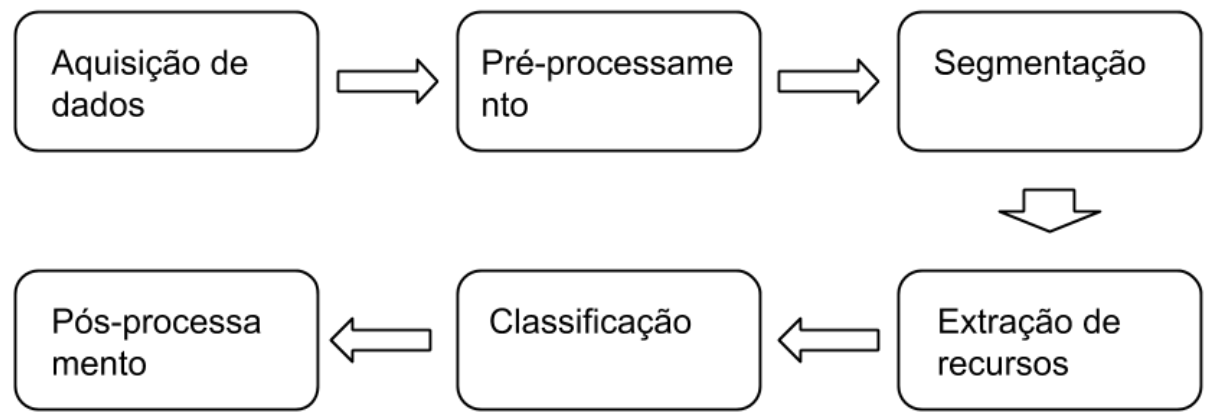
\includegraphics[width=1.0\textwidth]{Imagens/etapasocr} 
	\caption[Sequência de etapas em um sistema OCR.]{Sequência de etapas em um sistema OCR.}
\fonte{\citeonline{Goswami2013}}	
	\label{fig:tux_laplace}
\end{figure}

Segundo \citeonline{Goswami2013}, a primeira etapa é a aquisição de dados, que pode ser feita por meio de um escaneamento óptico, capaz de realizar a transformação de um documento físico em uma imagem digitalizada ou por uma câmera. Em seguida, a etapa de pré-processamento com a finalidade de melhorar o documento para aplicação da segmentação. Na etapa de segmentação os caracteres são separados e extraídos para serem identificados. E por fim, os caracteres são reconstruídos em palavras pela etapa de pós-processamento.

Na etapa de aquisição de dados, pode ser obtida uma imagem digital por meio de captura fotográfica. Na criação de um sistema de reconhecimento de caracteres on-line, é utilizado digitalizadores que capturam diretamente a escrita pela ordem dos traços e pela velocidade \cite{Goswami2013}.

Após a etapa de aquisição de imagem onde a imagem já está digitalizada, pode existir uma certa quantidade de imperfeições e ruídos \cite{Eikvil1993}. Desse modo, o pré-processamento tem como objetivo utilizar uma série de técnicas com o intuito de aperfeiçoar a imagem para as etapas decorrentes \cite{Goswami2013}. Dentre as diversas técnicas que podem ser aplicadas, as de maior importância são: normalização e redução de ruído. Normalização é considerada a etapa de mais relevância do pré-processamento, pois consegue obter caracteres de tamanho, rotação uniforme e inclinação \cite{Eikvil1993}. O objetivo da redução de ruído é solucionar problemas como segmentos de linhas desconectados, lacunas nas linhas, distorção e outras imperfeições por meio de métodos de filtragem, operações morfológicas, suavização e modelagem de ruído \cite{Goswami2013}. 
Na Figura 11 está representada a aplicação das técnicas de normalização e redução de ruído.

 \begin{figure}[h]
	\centering
	
\includegraphics[width=1.0\textwidth]{Imagens/norm_suav_caracter} 
	\caption[Normalização e redução de ruído de um caractere.]{Normalização e redução de ruído de um caractere.}
\fonte{\citeonline{Eikvil1993}}	
	\label{fig:tux_laplace}
\end{figure}

Segundo \citeonline{Eikvil1993}, a segmentação é o processo que determina os constituintes de uma imagem. Basicamente, a segmentação é executada em duas categorias: segmentação interna, que lida com a divisão de letras normalmente escritas de forma cursiva e a segmentação externa, na qual faz a divisão de unidades escritas como palavras, frases ou parágrafos \cite{Goswami2013}. Pode ocorrer nos componentes de dois caracteres adjacentes, uma sobreposição criando dificuldades na etapa de segmentação, por este motivo é de suma importância que esses caracteres sejam separados corretamente para que proporcione a identificação \cite{Bhatia2014}.

O objetivo da etapa de extração de características é extrair as características
essenciais de cada símbolo, onde no reconhecimento de pradrões é um dos problemas mais difíceis para os padrões de reconhecimento \cite{Eikvil1993}. A extração de características é composta por diversas técnicas e podem ser classificadas nos três seguintes grupos.

\begin{enumerate}
	\item Transformação global e expansão em série: As transformações e expansões em séries têm como principal foco a
redução da influência das rotações e translações que podem haver. Um sinal contínuo geralmente contém as informações necessárias para o propósito de classificação. Uma abordagem para representar um sinal é a combinação linear de uma sequência de funções bem definidas \cite{Goswami2013}. Os métodos mais comuns para transformação e expansão em série são as transformadas de Fourier, Gabor, Walsh, Haar, Hadamard, Hough e Karhunen-Loeve. Em sua maioria, se baseiam nas curvas que fazem o contorno dos caracteres, fazendo com que sejam muito sensíveis aos ruídos nas mesmas \cite{Eikvil1993}.
	\item Representação estatística: As técnicas de representação estatística são utilizadas na variação de estilo do caractere. Embora esse tipo de representação não permita a reconstrução da imagem original, ela é usada para reduzir o tamanho do conjunto de recursos, fornecendo alta velocidade e baixa compledixade \cite{Eikvil1993}. \citeonline{Eikvil1993} descreve os principais recursos estatísticos utilizados para a representação de caracter: Zoneamento, Travessias e Distâncias e Projeções.
	% EVERTON: no final, o que é "caracter"? Não seria "caractere"?
	
	\item Representação topológica e geométrica: Diversas propriedades globais e locais dos caracteres podem ser representadas por características geométricas e topológicas. De posse dessas informações, é possível identificar pontos de término, intersecções de linha, ranhuras, entre outras características. Em contraponto às outras técnicas anteriormente apresentadas, essas fornecem características tolerantes a ruídos e variações de estilo. No entanto, quando há translações e rotações não são tão efetivas quanto às demais \cite{ANDRADE2016}. 
\end{enumerate}



Para \citeonline{Eikvil1993}, a classificação é o processo de identificar cada caractere e atribuir a ele a sua correspondente classe de caracteres. Existem dois principais métodos diferentes para a classificação no reconhecimento de caracteres: análise teórica de decisão e estrutura física do caractere. 


Em análise teórica os métodos são usados quando a descrição do caractere pode ser representada numericamente por um vetor de características. Segundo \citeonline{Eikvil1993}, as principais abordagens para o reconhecimento utilizando teoria da decisão são: distância, classificadores mínimos, classificadores estatísticos e redes neurais.

Já na abordagem derivada das propriedades físicas, \citeonline{Eikvil1993} define métodos sintáticos entre as abordagens mais utilizadas. Classificação por métodos sintáticos medem a similaridade entre duas estruturas de componentes utilizando conceitos de gramática. A ideia é que cada classe tenha a sua própria gramática que defina a composição da gramática do caractere \cite{ANDRADE2016}. 




Na última etapa, após a resultante de um reconhecimento, \citeonline{Victor2017} diz que é realizado o método de agrupamento e a detecção e correção de erros na etapa de pós-processamento. O método de agrupamento nada mais é do que símbolos individuais convertidos em caracteres que são agrupados para formar palavras de acordo com a distância entre eles no documento. Os símbolos que são encontrados próximos o suficiente são agrupados, e os outros separadas em palavras. Essa associação de símbolos é, de fato, o processo de agrupamento. Segundo \citeonline{ANDRADE2016}, o agrupamento acaba sendo muito mais simples quando o texto reconhecido disserta poucas variações de tamanhos de fonte, e também com uma padronização de distâncias entre caracteres e palavras, ao contrário disso, pode aumentar muito a complexidade do agrupamento. Outro problema que podemos ter no processo são os textos inclinados.


Outra técnica utilizada no pós-processamento é a detecção e correção de erros, que emprega o uso de dicionários e regras de sintaxe para averiguar os conjuntos de caracteres agrupados \cite{Eikvil1993}. Segundo \citeonline{ANDRADE2016}, a abordagem do uso de dicionários tem sido a mais eficiente para a detecção e correção de erros. Dada uma palavra, a mesma é buscada no dicionário do idioma em evidência, se a palavra não se encontra no dicionário, um erro foi encontrado e pode ser corrigida a palavra por uma semelhante à incorreta.



\subsection{Bibliotecas de OCR}

As primeiras máquinas de reconhecimento eram todos dispositivos físicos de hardware. Atualmente essas máquinas ainda são utilizadas para aplicações específicas onde a velocidade é de grande importância, como por exemplo ordenação de cartas, leitura de cheques e verificação de passaportes (EIKVIL, 1993). Pelo fato de essas máquinas terem um custo de fabricação alto e com os avanços da computação, foi tornando possível a implementação de softwares de OCR que operam em computadores pessoais. Entretanto, existem algumas limitações para o sistema de OCR, especialmente em relação a velocidade e o tipo de caractere a ser lido (EIKVIL, 1993). 

% EVERTON: E de 94 pra cá? Novamente, sempre que cita ano e referências, são muito antigas.
Entre os anos de 1985 e 1994 foi desenvolvido pela empresa HP (Hewlett Packard), um sistema de OCR compatível com diversos sistemas operacionais chamado de Tesseract. No ano de 1996 ele teve a portabilidade para o sistema operacional Windows e logo em seguida em 1998 seu código foi reescrito da linguagem C para C++. Após seu funcionamento apresentar bons resultados, em 2005 a licença Apache foi liberada com a ideologia de software livre, tendo o desenvolvimento patrocinado pela Google e por desenvolvedores do mundo todo. Essa poderosa ferramenta pode reconhecer texto de até 60 diferentes idiomas. Embora o Tesseract seja uma aplicação de OCR gratuita, o resultado de sua aplicação em imagens digitais de documentos pode não conter todas as informações desejadas. Entretanto, existem outras aplicações modernas que conseguem desempenhar bons resultados na extração de texto de imagens, como por exemplo o Google Cloud Vision API e o Microsoft Vision API. Essas aplicações utilizam modelos de aprendizado de máquina capazes de extrair diversas características da imagem e possivelmente bons resultados na extração de texto.

% EVERTON: Não escreva como está neste início. Não é post ou tutorial. Fale da tecnologia diretamente. Quando você fala "atualmente", que época é? Evite estes termos.
Será apresentado na sequência, detalhes do SDK Firebase ML Kit (Firebase Machine Learn Kit) que é o SDK voltado a para dispositivos móveis da API Google Cloud Vision, que leva a experiência em aprendizado de máquina do Google para aplicativos Android e iOS em um pacote poderoso e fácil de usar \cite{CODELABS}. A API do Mobile Vision fornece uma estrutura para encontrar objetos em fotos e vídeos. A estrutura inclui detectores, que localizam e descrevem objetos visuais em imagens ou quadros de vídeo, e uma API orientada a eventos que rastreia a posição desses objetos em vídeo. Atualmente, a API do Mobile Vision inclui detectores de face , código de barras e texto , que podem ser aplicados separadamente ou em conjunto \cite{INTROMOBILEVISION}.

O pacote de visão inclui uma estrutura de funcionalidade de base comum e subpacotes para implementações de detectores específicos como detector de face, detector de código de barras e também detector de texto \cite{INTROMOBILEVISION}.

O ML Kit facilita a aplicação de técnicas de ML em seus aplicativos, trazendo as tecnologias ML do Google, como a API do Google Cloud Vision , o Mobile Vision e o TensorFlow Lite , juntos em um único SDK \cite{CODELABS}.

No processo de detecção e reconhecimento de texto em imagens, uma vez detectado, o reconhecedor determina o texto real em cada bloco e o segmenta em linhas e palavras. A API de texto detecta texto em idiomas latinos (francês, alemão, inglês, etc.) em tempo real no dispositivo.

O Reconhecedor de Texto segmenta o texto em blocos, linhas e palavras:

1 - Um bloco é um conjunto contíguo de linhas de texto, como um parágrafo ou coluna.

2 - Uma linha é um conjunto contíguo de palavras no mesmo eixo vertical.

3 - Uma palavra é um conjunto contíguo de caracteres alfanuméricos no mesmo eixo vertical.

A Figura 12 destaca exemplos de cada um deles em ordem decrescente. O primeiro bloco destacado, em ciano, é um bloco de texto. O segundo conjunto de blocos destacados, em azul, são linhas de texto. Finalmente, o terceiro conjunto de blocos destacados, em azul escuro, são as palavras \cite{MOBILEVISION}.

 \begin{figure}[h]
	\centering
	
	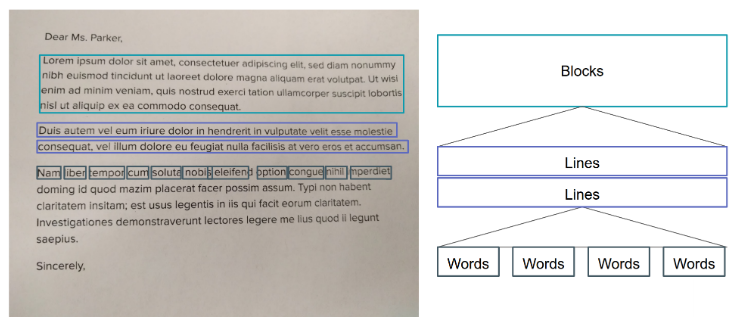
\includegraphics[width=1.0\textwidth]{Imagens/estruturatexto} 
	\caption[Reconhecimento de texto segmentado em texto em blocos, linhas e palavras.]{Reconhecimento de texto segmentado em texto em blocos, linhas e palavras.}
\fonte{\citeonline{MOBILEVISION}}	
	\label{fig:tux_laplace}
\end{figure}

\chapter{Metodologia} \label{cap:metod}

Nesse capítulo é descrita a metodologia utilizada para o desenvolvimento deste projeto. São descritas as etapas do projeto e os principais fundamentos e tecnologias a serem empregados.

O trabalho será composto por seis etapas:

\begin{enumerate}
\item Projetar e preparar a estrutura física.
\item Modelar o sistema.
\item Projetar e implementar o sistema de comunicação.
\item Projetar e construir o sistema embarcado.
\item Projetar e implementar o sistema de controle.
\item Idealizar e conduzir experimentos reais de teste de navegação.
\end{enumerate}

%PARA AS ETAPAS ACREDITO QUE POSSA COMEÇAR ASSIM: NA ETAPA RELACIONADA AO PROJETO E PREPARAÇÃO.....E IR VARIANDO DE UM PARÁGRAFO PARA O OUTRO, PARA NÃO FICAR REPETITIVO.
\noindent{\bf Etapa 1:} essa etapa será destinada ao projeto, aquisição e montagem da estrutura física do quadricóptero %?????? ACHO QUE ISSO NÃO É SEU TRABALHO..PAREI A LEITURA AQUI E CONTINUAREI APÓS SEU RETORNO. A estrutura é composta basicamente por um chassi, quatro motores, quatro hélices e uma bateria. Deverão ser analisados os recursos disponíveis no mercado ou passíveis de empréstimo capazes de satisfazer os requisitos do sistema. Ao final desta etapa, a estrutura deverá ser testada com o sistema eletrônico de um quadricóptero de controle remoto comercial, a fim de verificar suas capacidades básicas de voo.

\noindent{\bf Etapa 2:} nessa fase será feita a modelagem matemática da estrutura física desenvolvida na etapa anterior. Essa modelagem é necessária para o projeto do sistema de controle que será desenvolvido na etapa 5. Apesar de ter um grande foco teórico, também serão necessários testes empíricos.

\noindent{\bf Etapa 3:} aqui deverá ser desenvolvido o sistema de comunicação. Haverá dois canais de comunicação: um principal (quadricóptero-estação base), para definição de objetivos e coleta de dados, e um secundário (quadricóptero-controle remoto), de emergência, para que um humano possa assumir o controle. Deverão ser analisadas as tecnologias disponíveis, custo de implementação e integração com o sistema embarcado, a estação base e o controle remoto.

\noindent{\bf Etapa 4:} essa etapa é destinada o projeto e construção de um sistema embarcado microcontrolado para realização das funções do quadricóptero. O sistema deve ser capaz de realizar todas as tarefas em tempo real e de forma autônoma. Suas tarefas incluem: leitura dos sensores, comunicação, execução do sistema de controle de estabilidade e acionamento dos motores. Pode ser escolhido um sistema comercial, desde que atenda ao requisitos e que ofereça total acesso ao microcontrolador, ou pode ser desenvolvido um.

%O canal principal será entre o quadricóptero e uma estação base. A estação base enviará rotas de voo ou objetivos para o quadricóptero, e coletará dados dos sensores e estados internos. O canal secundário, ou de emergência, será estabelecido entre um controle remoto e o quadricóptero. Sua função é permitir que, em casos de mal funcionamento, risco de dano ao veículo ou a pessoas ao redor, um piloto externo possa assumir o controle e aterrissá-lo em uma posição segura.

\noindent{\bf Etapa 5:} nessa fase deverá ser projetado e implementado um sistema de controle de estabilidade e desvio de obstáculos. Diversas técnicas de controle já foram analisadas em outros projetos, cada uma apresentando vantagens e desvantagens, de acordo com as características do ambiente de estudo. Com base nesses trabalhos deverão ser escolhidas uma ou mais técnicas para utilização. Baseado na modelagem matemática desenvolvida na etapa 2, softwares matemáticos poderão ser utilizados para auxiliar no projeto do controlador, realizando simulações do funcionamento do sistema antes da implementação no sistema embarcado. Testes reais deverão ser realizados.

\noindent{\bf Etapa 6:} por fim, deverão ser conduzidos testes para verificar o funcionamento completo do veículo e validar os objetivos deste projeto.
\chapter{Recursos de Hardware e Software} \label{cap:recur}

Neste capítulo serão apresentados os principais recursos de \textit{hardware} e \textit{software} utilizados nesse projeto, bem como a origem destes recursos.


\section{Recursos de Hardware} \label{sec:recurhard}

Os recursos de \textit{hardware} necessários englobam o quadricóptero, o sistema de comunicação e a estação base.

O quadricóptero pode ser divido em duas partes: estrutura física e placa de controle. Os componentes da estrutura física são:

\begin{itemize}
\item 1x Chassi de 45cm diâmetro 
\item 4x Motor brushless 5000kV 
\item 4x Hélice 9x4,7 GWS 
\item 4x \sigla{ESC}{Eletronic Speed Control} 30A 
\item 1x Bateria 4000mAh 7,4V
\end{itemize}

estes componentes foram emprestados pelo prof. Hugo Vieira, orientador desse trabalho. Também foi emprestada uma placa de controle, chamada ``KK multicopter'', porém essa é uma placa de baixo desempenho e espera-se substituí-la por uma melhor. O desejável seria construir a própria placa de controle, porém devido ao encapsulamento \sigla{SMD}{Surface Mounted Device} utilizado nos sensores MEMS, a montagem dessas placas requer o uso de equipamentos específicos, inviáveis para esse projeto.

Até o momento não há disponibilidade de nenhum dos componentes do sistema de comunicação, todos deverão ser adquiridos. Eles são:

\begin{itemize}
\item 2x Módulo transceptor de RF
\item 1x USB \textit{dongle}
\item 1x Rádio controle 4 ou mais canais
\item 1x Receptor 4 ou mais canais
\end{itemize}

A estação base é um computador, desktop ou portátil, recente, com sistema operacional Windows ou Linux. Será usado um computador próprio.


\section{Recursos de Software}

Alguns recursos de software utilizados dependerão das alternativas de hardware escolhidas e só poderão ser definidas posteriormente. Inicialmente serão utilizados os seguintes:

\begin{itemize}
\item Matlab ou Octave: simulações do sistema de controle, coleta de dados do quadricóptero. Disponíveis na UTFPR e gratuito, respectivamente.
\item Eagle: criação de diagramas eletrônicos e placas de circuito impresso. Gratuito.
\item Astah community ou Dia: edição de diagramas UML e fluxogramas. Ambos gratuitos.
\end{itemize}








\chapter{Viabilidade e Cronograma Preliminar} \label{cap:viabi}

Neste capítulo será avaliada a viabilidade do projeto e será apresentado um cronograma preliminar de desenvolvimento.


\section{Viabilidade}

Como descrito no capítulo anterior, os principais recursos para a elaboração do projeto foram emprestados, para os de hardware, ou são gratuitos, para os de software. Resta para aquisição apenas os componentes da comunicação e da placa controladora. O gasto estimado para aquisição dos componentes e conclusão do projeto é de 300 reais, contanto que não ocorram danos no desenvolvimento, o que é completamente viável.


\section{Cronograma Preliminar}

A Tabela \ref{tab:crono} apresenta um cronograma preliminar do desenvolvimento do \sigla{TCC}{Trabalho de Conclusão de Curso}. Na sua elaboração foi considerado que o autor continuará o desenvolvimento no semestre seguinte, junto com a disciplina de TCC 2.

\begin{table}[!htb]
\caption{Cronograma} \label{tab:crono}
\begin{center}
	\begin{tabularx}{\textwidth}{|X|c|c|}
	\hline
	\textbf{Etapa} & \textbf{Data de início} & \textbf{Data de término} \\
	\hline
	Elaboração da proposta de TCC &
	11/12/12 & 19/03/13 \\
	\hline
	Entrega da proposta de TCC &
	26/03/13 & 26/03/13 \\
	\hline
	Elaboração do plano de projeto de TCC &
	26/04/13 & 23/04/13 \\
	\hline
	Entrega do plano de projeto de TCC &
	08/05/13 & 08/05/13 \\
	\hline
	Elaboração da monografia de TCC &
	03/06/13 & 10/10/13 \\
	\hline
	Projetar e montar a estrutura física &
	03/06/13 & 16/06/13 \\
	\hline
	Modelar o sistema &
	17/06/13 & 30/06/13 \\
	\hline
	Projetar e implementar o sistema de comunicação &
	01/07/13 & 28/07/13 \\
	\hline
	Projetar e construir o sistema embarcado &
	01/07/13 & 28/07/13 \\
	\hline
	Projetar e implementar o sistema de controle &
	29/07/13 & 01/09/13 \\
	\hline
	Idealizar e conduzir experimentos reais de teste de navegação &
	02/09/13 & 06/10/13 \\
	\hline
	Entrega da monografia e  defesa do TCC &
	11/10/13 & 11/10/13 \\
	\hline	
	\end{tabularx}
\end{center}
\end{table}
\chapter{RESULTADOS E Discussões}\label{ch:intro}
Utilizando os materiais e métodos previamente apresentados, neste capítulo serão
apresentados e discutidos os resultados obtidos a partir dos experimentos abordados na base de imagens criada, assim como comparações com os efeitos de processamento de imagens aplicados na base de imagens coletada. Os resultados serão apresentados na ordem de imagens classificadas em ambiente de luminosidade favoráveis até as imagens capturadas em ambiente noturno.


As métricas apresentadas foram calculadas obtendo-se uma média de acertividade do resgate correto dos caracteres do nome do medicamento em questão, analisando a quantidade de caracteres e quantidade de resgates corretos.

 No decorrer da criação da base de imagens, foi constatado que o dispositivo celular Samsung J2  não possui boa captura de imagens em ambientes com baixa luminosidade, mas ainda assim optou-se por continuar com a captura de imagens e os testes, pelo fato de poder reproduzir uma situação real, que pode ocorrer com futuros usuários da aplicação em estudo.
 
Os testes foram realizados e comparados entre as categorias de imagens, perspectivas e entre as técnicas de processamento de imagem. Os testes foram encerrados quando três testes consecutivos da mesma categoria de imagens não obtiveram resgates de pelo menos 3 caracteres corretos e sequentes, o que impossibilitou o próximo passo, que é a recuperaração dos registros na base de dados descritiva dos medicamentos.

%EVERTON: O usuário precisará ter no dispositivo dele a base de todas as imagens?
Em todos os experimentos que serão apresentados, foi necessário importar as fotos do banco de imagens para o projeto como forma de asset, que é a forma correta onde um aplicativo de celular identifica e caracteriza uma imagem internamente para importação. Como forma de simplificar posteriormente as buscas na base de informações de remédios, foram ignorados os acentos, o que não impactará nos resultados do OCR demonstrados a seguir. Dessa maneira, caso o OCR identifique alguma letra que possua acento, é realizado um pós processamento no texto para que a consulta seja feita sem acentos e caracteres especiais, visando deixar a busca simplificada e com um poder acertivo maior.

\section{MANIPULAÇÃO DOS DADOS COLETADOS}

Segundo o Portal da \citeonline{PORTALANVISA}, desde o ano 2000 até 05/08/2019, 5.723 medicamentos genéricos foram registrados. Destes, 2.398 registros foram cancelados, restando 3.325 medicamentos genéricos com registros válidos. Em base dessa informação, pensando em trabalhos futuros e pensando em ganho de desempenho no dispositivo celular, foi optado por manipular os dados via \textit{JSON}, viabilizando de forma mais dinâmica o uso de banco de dados não relacionais, chamados de NoSQL, que trabalham diretamente com arquivos JSON.

Os dados coletados para este trabalho foram capturados manualmente do bulário da Anvisa e % -> escritos no salvos <- % no tipo JSON para facilitar a busca detalhada pela lista de objetos criadas do tipo Medicamento, onde possui as seguintes chaves de identificação:

\begin{lstlisting}[firstnumber=1]
{
  "medicamentos": [
      {"id": 1},
      {"nome": "descricao"},
      {"principios_ativos": "descricao"},
      {"contra_indicacoes": "descricao"},
      {"tipo_medicamento": "descricao"},
      {"data": "descricao"}
    ]
}
\end{lstlisting}
\fonte{Autoria Própia.}


Com retorno obtido do OCR Firebase MLKit, é possível obter os textos em blocos, linhas e palavras, conforme descrito na sessão 2.5.2, possibilitando realizar uma rápida busca no documento \textit{JSON} local. Por este motivo, foi elaborado um processo com 6 algoritmos de pós processamento dos dados, no intuito de efetuar uma busca mais refinada e acertiva dos dados coletados do OCR na base de dados JSON, que são:

\begin{enumerate}
  \item Limpeza dos dados coletados;
  \item Busca simples por palavras;
  \item Substituição de números visualmente similares a letras;
  \item Busca por palavras formatadas;
  \item Busca contendo a metade das letras iniciais das palavras;
  \item Busca contendo a metade das letras finais de cada palavra.
\end{enumerate}

%EVERTON: Você usa muito feito. Feito é fazer, construir. Procure melhorar esta situação no documento.
Na primeira etapa, algumas palavras padrões foram identificadas durante o estudo das caixas de medicamento como por exemplo: "VENDA SOB PRESCRIÇÃO MÉDICA", "50 mg", "Uso Oral", "Uso adulto" e "Contém 20 comprimidos". Essas palavras serão excluídas neste trabalho, porém elas podem servir de informações adicionais e podem ser relevantes para um sistema mais criterioso em trabalhos futuros.

Supondo que uma caixa de medicamento não contenha mais de 50 palavras, na segunda etapa do processo foi analisado que se faz viável a comparação de todas as palavras encontradas com todos os registros de chave de valor "nome" do documento JSON. Mesmo que seja encontrado algum registro, será efetuado a terceira etapa.

Na terceira etapa, é feito um segundo refinamento das informações nas palavras encontradas, se possuir caracteres iguals ao número 0, substituir pela letra "O", número 1 pela letra "L", número 4 pela letra "A" e também o número 7 pela letra "T", devido ao seu alto grau de semelhança visual para o OCR. 

Após feito a troca dos caracteres, será feita uma nova busca na base de dados JSON, passando palavra por palavra que representa a quarta tarefa da lista. Caso não seja encontrado nenhum registro, o algoritmo % COMO ASSIM?? interpretará o quinto passo, que é a separação da palavra ao meio, formando 2 partes, do início da palavra até a metade e da metade até o final. Fazendo então ser possível a busca novamente na base por medicamentos que contenham essa sequência de letras na chave "nome" do documento JSON.

A cada Medicamento encontrado nas etapas, o medicamento é inserido em uma lista que por fim será apresentada para o usuário, retornando apenas os medicamentos distintos encontrados. Caso haja mais de um medicamento encontrado na base, será apresentado uma lista simples, para que o usuário selecione o medicamento correto.


\section{Experimento sem manipulação de imagem}
Os resultados apressentados na Tabela \ref{tab:exp_sem_filtro}, são referentes às imagens originais submetidas ao OCR, sem nenhum tipo de tratamento de imagem. A coluna sem processamento dos dados, está representada por "SP" e a coluna com o pós processamento de dados, está representada por "CP".


\begin{table}[]
\caption{Experimento sem aplicar filtro nas fotos}
\label{tab:exp_sem_filtro}
\centering
\begin{tabular}{llccc}
\hline
Categoria          & Tamanho    & Tempo (sec) & SP \%  & CP \% \\ \hline
Boa luminosidade   & 76,8 MB & 72     & 100 & 100         \\
Baixa luminosidade & 104 MB & 91     & 83,33 & 100         \\
Ambiente externo   & 88,9 MB & 80     & 100 & 100         \\
Noturnas sem flash & 82,9 MB & 78     & 83,33& 100         \\
Noturnas com flash & 96,7 MB & 87     & 83,33 & 100         \\ \hline
\end{tabular}
\fonte{Autoria Própria.}	
	\label{fig:exp_sem_filtro}
\end{table}

Foi identificado 


\section{EXPERIMENTO APLICANDO efeito DE ESCALAS EM CINZA}
%EVERTON: Não é primeira pessoa
Para aplicar o filtro de imagem em escalas de cinza, foi necessário implementar um algoritmo para tal função. Como estamos manipulando um objeto do tipo \textit{File} (arquivo) da galeria, foi necessário decodificar o \textit{File} e transformar para um objeto do tipo textit{Image}. 

Para otimizar tempo e recurso de memória do celular que acabou sendo insuficiente, foi necessário fazer uma transformada no tamanho da imagem, para altura igual a 600 e largura igual a 600. Com o array de bits gerado da imagem, foi possível iniciar a conversão da imagem para escala de cinza, conforme figura \ref{fig:greyscale}, deixando assim, a imagem em escala de cinza pronta para ser aplicada ao OCR.


% Deixo essa imagem? Não consegui transformar para pseudo código


 \begin{figure}[h]
	\centering
	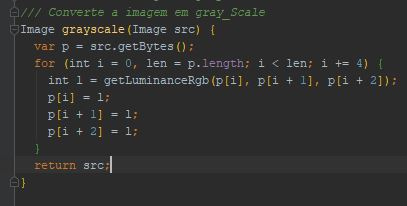
\includegraphics[width=0.6\textwidth]{Imagens/greyscale.JPG} % <- formatos PNG, JPG e PDF
	\caption[Algorítmo de conversão em escalas de cinza.]{Algorítmo de conversão em escalas de cinza.}
\fonte{Autoria Própria.}%citaç\~ao do livro onde pegou a figura	
	\label{fig:greyscale}
\end{figure}

Os resultados do experimento de pré processamento aplicando efeito de escalas em cinza na imagem, são apressentados na Tabela \ref{tab:exp_sem_filtro}.

\begin{table}[]
\caption{Experimento aplicando filtro de escalas em cinza.}
\label{tab:exp_grey_scale}
\centering
\begin{tabular}{llccc}
\hline
Categoria          & Tamanho    & Tempo (sec) & SP  & CP \% \\ \hline
Boa luminosidade   & 76,8 MB & 164     & 77 & 100         \\
Baixa luminosidade & 104 MB & 211     & 45 & 83,3         \\
Ambiente externo   & 88,9 MB & 181     & 77 & 100         \\
Noturnas sem flash & 82,9 MB & 600+     & 0& 0         \\
Noturnas com flash & 96,7 MB & 474     & 16,6 & 16,6         \\ \hline
\end{tabular}
\fonte{(Autoria Própria)}	
	\label{fig:exp_grey_scale}
\end{table}



\section{EXPERIMENTO APLICANDO efeito DE Sobel}

Para aplicar o efeito de Sobel na imagem, como proposto na sessão de materiais e métodos, foi necessário implementar um algoritmo para tal função. Também neste caso, como estamos manipulando um objeto do tipo \textit{File} da galeria, foi necessário decodificar o \textit{File} e transformar para um objeto do tipo \textit{Image}. Para otimizar tempo e recurso de memória, foi necessário fazer uma transformada no tamanho da imagem, para altura igual a 600 e largura igual a 600. Com o array de bits gerado da imagem, foi possível iniciar a conversão da imagem aplicando o filtro de Sobel. Deixando assim, a imagem com filtro de Sobel pronta para ser manipilada pelo OCR. 

\begin{table}[]
\caption{Experimento aplicando filtro de Sobel.}
\label{tab:exp_sobel}
\centering
\begin{tabular}{llccc}
\hline
Categoria          & Tamanho    & Tempo (sec) & SP\%  & CP \% \\ \hline
Boa luminosidade   & 76,8 MB & 451     & 0 & 0         \\
Baixa luminosidade & 104 MB & 570     & 0 & 0         \\
Ambiente externo   & 88,9 MB & 514     & 0 & 0         \\
Noturnas sem flash & 82,9 MB & 600+     & 0& 0         \\
Noturnas com flash & 96,7 MB & 600+     & 0 & 0         \\ \hline
\end{tabular}
\fonte{(Autoria Própria)}	
\end{table}

Como demonstrado na Tabela \ref{tab:exp_sobel}, houve uma grande complicação para processamento da imagem, tanto para a conversão quanto para o OCR de efetuar a extrassão dos caracteres nas imagens.

\chapter{CONSIDERAÇÕES FINAIS}\label{ch:intro}
Neste capítulo são resumidas as principais consideracões finais acerca do trabalho, bem como suas contribuicões sociais. Também é abordado possíveis trabalhos futuros para melhorar e dar continuidade ao objetivo de utilizar tecnicas de processamento de imagem juntamente com OCR no auxílio de uma classe social de idosos que vem crescendo continuamente no Brasil.


\section{CONCLUSÃO}

Este trabalho mostrou que é possível desenvolver técnicas de reconhecimento de caracteres em um ambiente offline acopladas a aplicativos, sendo possível auxiliar a população no processo medicamentoso. Com uma foto de boa qualidade, luminosidade e resolução maior que 5mp, é possível extrair o nome e informações adicionais da embalagem do medicamento em questão em pouco menos de 3 segundos, dando um amplo acesso a possibilidades para se trabalhar com esse tipo de dado e solucionando problemas sociais e empresariais.

Com o estudo implementado neste trabalho, é possível levar informação a uma grande parcela da população brasileira que por vezes não dispõe de capacidades visuais para ler letras miúdas de uma bula, pessoas não analfabetizadas, pessoas sem acesso a internet e até mesmo um aplicativo de auto ajuda para o dia a dia de agentes da saúde, que muitas vezes se encontram em locais remotos sem acesso a informações.  

Para o celular, além de complexo a nível de hardware limitado, efetuar técnicas de processamento de imagens se mostrou causar uma demora significativa para a tarefa e sendo menos eficiente do que imagens sem técnicas de processamento.

No conjunto de imagens expostas à técnicas de processamento de imagem, as imagens com pré processamento obtiveram menores taxas de acertividade e um tempo maior de processamento, uma vez que os recursos de processamento do aparelho celular são limitados para tal função. Por estes motivos, foi possível observar que o OCR da Google se saiu melhor em fotos de uso real do dia a dia.

Os testes realizados foram efetuados com caixas de medicamentos aleatórios, diferentes tamanhos, perspectivas, cores e tonalidades de contraste, o que não foi um grande desafio para o tema proposto.

Visando trabalhos futuros com consultas de bases de dados mais complexas e externas do celular, foi implementado a regra de estrutura de dados manipulando JSON, onde os dados serão muito melhor trafegados pela rede. Outro lado positivo estudado neste trabalho, foi o OCR do Firebase MLKIT, que apresentou um resultado excelente no resgate de caracteres, chegando quase a perfeição do reconhecimento dos caracteres a nível de nome do medicamento.

\section{trabalhos futuros}


Para possíveis trabalhos futuros baseados neste, se indica:

\begin{enumerate}
  \item Aplicar outros SDK de OCR para possíveis melhores resultados.
  \item Melhorar o algoritmo de busca em lista para ter uma melhor eficácia na identificação do medicamento, caso o OCR venha errar sequência de 3 letras ou mais da palavra do medicamento em questão.
  \item Generalizar o tema proposto, sendo possível trabalhar com diferentes categorias de imagens e com diferentes problemas sociais.
  \item Criar uma base de dados externa para consultas complexas que possa retornar mais informações do medicamento em questão ou até mesmo apresentar informações mais pertinentes, assim como cadastro de medicamentos não regulamentados pela Anvisa na base de dados descritiva dos medicamentos.
\end{enumerate}





%---------- Referencias ----------
\clearpage % this is need for add +1 to pageref of bibstart used in 'ficha catalografica'.
\label{bibstart}
\bibliography{bibliografia} % geracao automatica das referencias a partir do arquivo bibliografia.bib
\label{bibend}



% --------- Ordenacao Afabetica da Lista de siglas --------
%\textbf{* Observa\c{c}\~oes:} a ordenacao alfabetica da lista de siglas ainda nao eh realizada de forma automatica, porem
% eh possivel se de realizar isto manualmente. Duas formas:
%
% ** Primeira forma)
%    A ordenacao eh feita com o auxilio do comando 'sort', disponivel em qualquer
% sistema Linux e UNIX, e tambem em sistemas Windows se instalado o coreutils (http://gnuwin32.sourceforge.net/packages/coreutils.htm)
% comandos para compilar e ordenar, supondo que seu arquivo se chame 'dissertacao.tex':
%
%      $ latex dissertacao
%      $ bibtex dissertacao && latex dissertacao
%      $ latex dissertacao
%      $ sort dissertacao.lsg > dissertacao.lsg.tmp
%      $ mv dissertacao.lsg.tmp dissertacao.lsg
%      $ latex dissertacao
%      $ dvipdf dissertacao.dvi
%
%
% ** Segunda forma)
%\textbf{Sugest\~ao:} crie outro arquivo .tex para siglas e utilize o comando \sigla{sigla}{descri\c{c}\~ao}.
%Para incluir este arquivo no final do arquivo, utilize o comando \input{arquivo.tex}.
%Assim, Todas as siglas serao geradas na ultima pagina. Entao, devera excluir a ultima pagina da versao final do arquivo
% PDF do seu documento.


%-------- Citacoes ---------
% - Utilize o comando \citeonline{...} para citacoes com o seguinte formato: Autor et al. (2011).
% Este tipo de formato eh utilizado no comeco do paragrafo. P.ex.: \citeonline{autor2011}

% - Utilize o comando \cite{...} para citacoeses no meio ou final do paragrafo. P.ex.: \cite{autor2011}



%-------- Titulos com nomes cientificos (titulo, capitulos e secoes) ----------
% Regra para escrita de nomes cientificos:
% Os nomes devem ser escritos em italico, 
%a primeira letra do primeiro nome deve ser em maiusculo e o restante em minusculo (inclusive a primeira letra do segundo nome).
% VEJA os exemplos abaixo.
% 
% 1) voce nao quer que a secao fique com uppercase (caixa alta) automaticamente:
%\section[nouppercase]{\MakeUppercase{Estudo dos efeitos da radiacao ultravioleta C e TFD em celulas de} {\textit{Saccharomyces boulardii}}
%
% 2) por padrao os cases (maiusculas/minuscula) sao ajustados automaticamente, voce nao precisa usar makeuppercase e afins.
% \section{Introducao} % a introducao sera posta no texto como INTRODUCAO, automaticamente, como a norma indica.


\end{document}
